\section{Ruisreductie}

\subsection{Academisch voorbeeld zonder ruis}

Bij wijze van opwarming starten we met de wavelet decompositie van de functie $ \mathbb{R}  \to \mathbb{R}: x \mapsto \exp(x)$. 
Dit is een gladde functie die bovendien analytisch is. 
Voor onze analyse werden de de exponenti\"ele functie equidistant bemonster op het interval $ [0,1] $ met $ 256 $ punten.
Deze data werd nadien geanalyseerd met behulp van 3 verschillende wavelet transformaties, de haar wavelet, de daubechie wavelet van orde 4 en de daubechie wavelet van orde 45.
Elk van deze transformaties werd uitgevoerd tot niveau 4, dit maakt dus dat het signaal zal worden opgesplitst ten opzichte van 5 verschillende basissen.  
De resultaten van dit experiment zijn samen gevat in Figuur \ref{fig:exp_noNoise}.
In de linker kolom van de figuur zijn de coefficienten van de transformatie uitgezet.
In de rechter kolom is telkens de benadering van de exponenti\"ele functie in elke basis uitgezet.
Hierbij is de onderste curve de benadering in $ W_1 $, die daar boven de benadering in $ W_2 $ en zo voort.
De bovenste grafiek is dan de benardering van de exponenti\"ele functie in de ruimte $ V_4 $.

Wat meteen opvalt is dat de coefficienten van de lage frequenties (links in de coefficienten vector) het grootst zijn.
Dit is volledig volgens de verwachting, de exponentiele funtie is een gladde functie en bevat dus voornamelijk lage frequenties.
Een tweede bemerking is dat voor de hogere orde wavelets de coefficienten aan de randen groter worden.
Dit is het gevolg van het breder worden van de wavelet, hierdoor zal het eind effect verstrekt worden.

Vervolgens kunnen we zien naar de kwaliteit van de benaderingen in de opeen volgde vector ruimtes, zoals gegeven in de rechter kolom.
Hier is het duidelijk dat een hogere orde benadering niet meteen een snellere convergentie geeft.
Dit is opnieuw het gevolg van het bredere karakter van de hogere orde wavelets.
Over het algemeen is de beste benadering bekomen door de daubechie wavelte van orde 2.
Het eind effect is het kleinste voor de haar wavelet.

\subsection{Academisch voorbeeld met ruis}

In een tweede test word er ruis toegevoegd aan de gladde functie exponenti\"ele functie.
Deze ruis is witte ruis met een standaard afwijking van 0.1.
Om de invloed van de ruis op de wavelet coefficienten duidelijk te maken zijn de coefficienten weergegeven in 
figuur \ref{fig:exp_Noise_noise_10}.
De invloed van de witte ruis in het tijddomein geeft  een verstoring van witte ruis op de coefficienten van de versrchillende wavelet transformaties.
De verstoring kan makkelijk worden verwijderd aan de hand van een treshold waarder te gebruiken.
Deze methode is besproken in de opgaven en zal dus niet verder worden toegelicht.
Enkel de resultaten en toepassingen zullen worden besproken.

De fout als functie van de threshold waarden is weergeven in figuur \ref{fig:error_exp_haar_10} tot \ref{fig:error_exp_db45_10}.
Uit deze drie figuren is het duidelijk dat er een fundamenteel verschil optreed tussen de zachte threshold functie en de twee andere.
De verklaring hiervoor is dat de zachte threshold functie elke waarden zal wijzigen, zelfs de waarden ver boven de threshold.
Om dit te illustreren zijn de drie threshold functies weergegeven in Figuur \ref{fig:Threshold}.

Om dit deel af te sluiten is in figuur \ref{fig:Optimale_ruisReductie} de optimale ruis reductie weergegeven.
Deze reducties maakt gebruik van daubechie wavelet van orde 2 en een threshold waarden van 0.4 met  de zachte treshold functie.


\paragraph{Tussenliggende waarden bepalen}

\dots Iets met de basis wavelet bepalen in het punt  en zo kan je het doen. Ik denk dat dit iets te maken heeft met een wavelet interpolatie.


\begin{figure}
    \centering
     \begin{subfigure}[b]{0.45\textwidth}
            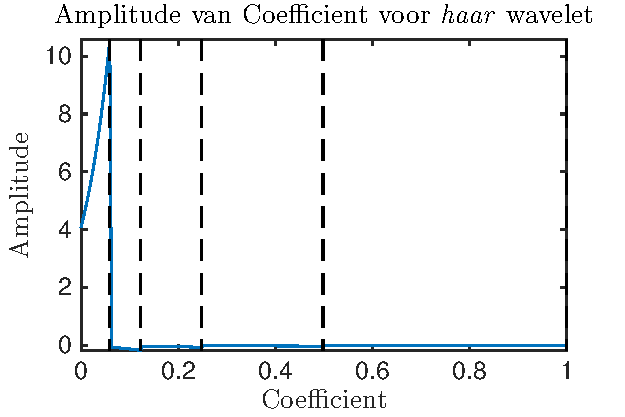
\includegraphics[width=\textwidth]{../src/denoising/haar_noNoise/coef_exp_haar_4}
            \caption{Met tekst beschadiging}
            \label{fig:tiger}
        \end{subfigure}
        ~ %add desired spacing between images, e. g. ~, \quad, \qquad, \hfill etc. 
        %(or a blank line to force the subfigure onto a new line)
        \begin{subfigure}[b]{0.45\textwidth}
            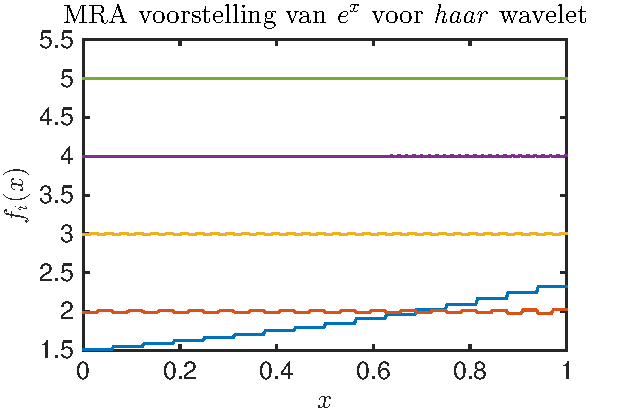
\includegraphics[width=\textwidth]{../src/denoising/haar_noNoise/MRA_exp_haar_4}
            \caption{Na de reconstructie}
            \label{fig:mouse}
        \end{subfigure}
    \begin{subfigure}[b]{0.45\textwidth}
        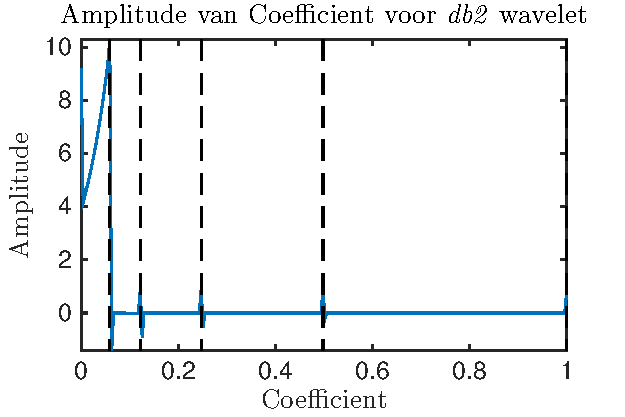
\includegraphics[width=\textwidth]{../src/denoising/db2_noNoise/coef_exp_db2_4}
        \caption{Met tekst beschadiging}
        \label{fig:tiger}
    \end{subfigure}
    ~ %add desired spacing between images, e. g. ~, \quad, \qquad, \hfill etc. 
    %(or a blank line to force the subfigure onto a new line)
    \begin{subfigure}[b]{0.45\textwidth}
        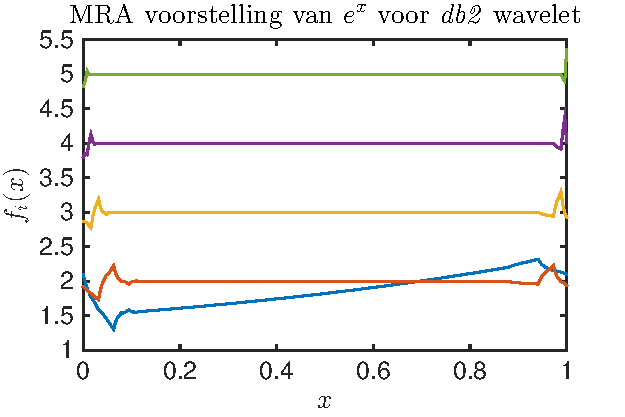
\includegraphics[width=\textwidth]{../src/denoising/db2_noNoise/MRA_exp_db2_4}
        \caption{Na de reconstructie}
        \label{fig:mouse}
    \end{subfigure}
    \begin{subfigure}[b]{0.45\textwidth}
        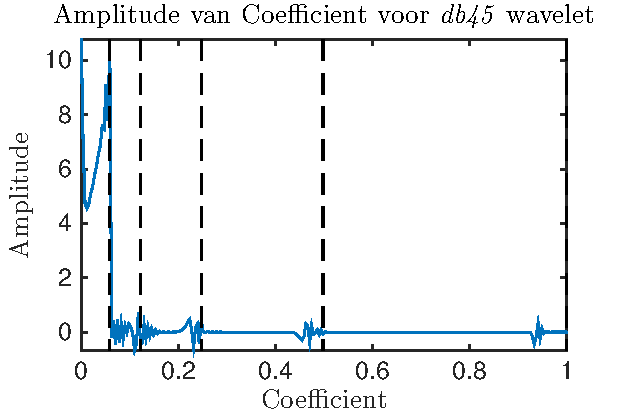
\includegraphics[width=\textwidth]{../src/denoising/db45_noNoise/coef_exp_db45_4}
        \caption{Met tekst beschadiging}
        \label{fig:tiger}
    \end{subfigure}
    ~ %add desired spacing between images, e. g. ~, \quad, \qquad, \hfill etc. 
    %(or a blank line to force the subfigure onto a new line)
    \begin{subfigure}[b]{0.45\textwidth}
        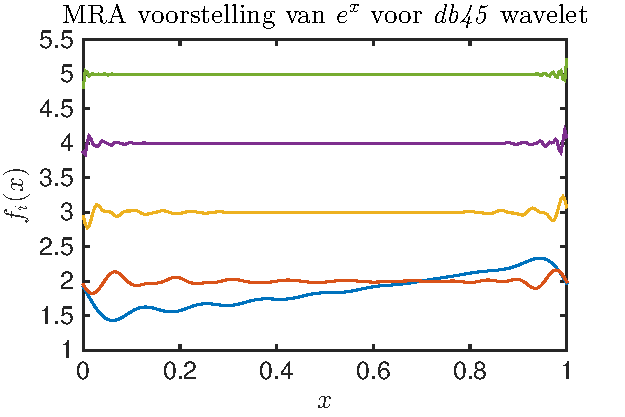
\includegraphics[width=\textwidth]{../src/denoising/db45_noNoise/MRA_exp_db45_4}
        \caption{Na de reconstructie}
        \label{fig:mouse}
    \end{subfigure}
    \caption{Pictures of lena}\label{fig:exp_noNoise}
\end{figure}


\begin{figure}
    \centering
     \begin{subfigure}[b]{0.45\textwidth}
            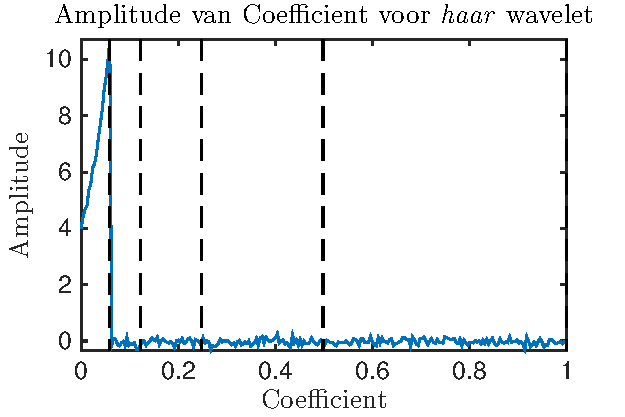
\includegraphics[width=\textwidth]{../src/denoising/haar_Noise/coef_exp_haar_4_noise_10}
            \caption{Met tekst beschadiging}
            \label{fig:tiger}
        \end{subfigure}
        ~ %add desired spacing between images, e. g. ~, \quad, \qquad, \hfill etc. 
        %(or a blank line to force the subfigure onto a new line)
        \begin{subfigure}[b]{0.45\textwidth}
            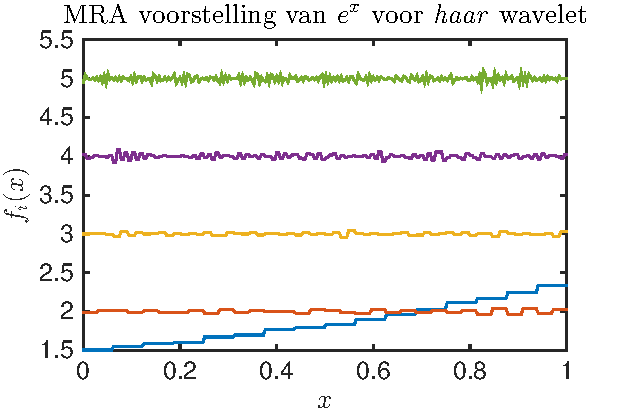
\includegraphics[width=\textwidth]{../src/denoising/haar_Noise/MRA_exp_haar_4_noise_10}
            \caption{Na de reconstructie}
            \label{fig:mouse}
        \end{subfigure}
    \begin{subfigure}[b]{0.45\textwidth}
        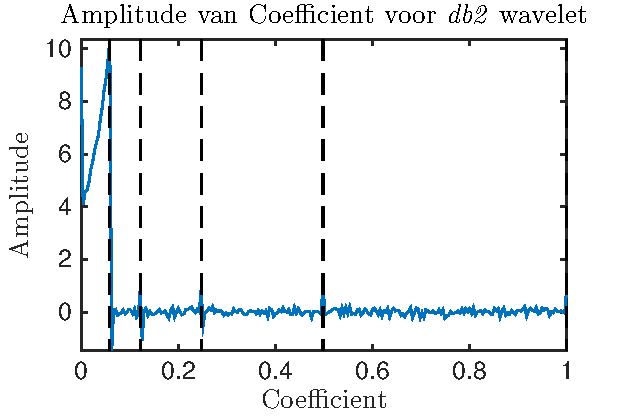
\includegraphics[width=\textwidth]{../src/denoising/db2_Noise/coef_exp_db2_4_noise_10}
        \caption{Met tekst beschadiging}
        \label{fig:tiger}
    \end{subfigure}
    ~ %add desired spacing between images, e. g. ~, \quad, \qquad, \hfill etc. 
    %(or a blank line to force the subfigure onto a new line)
    \begin{subfigure}[b]{0.45\textwidth}
        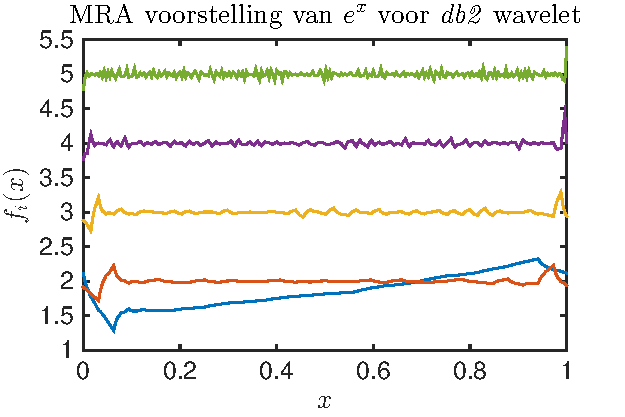
\includegraphics[width=\textwidth]{../src/denoising/db2_Noise/MRA_exp_db2_4_noise_10}
        \caption{Na de reconstructie}
        \label{fig:mouse}
    \end{subfigure}
    \begin{subfigure}[b]{0.45\textwidth}
        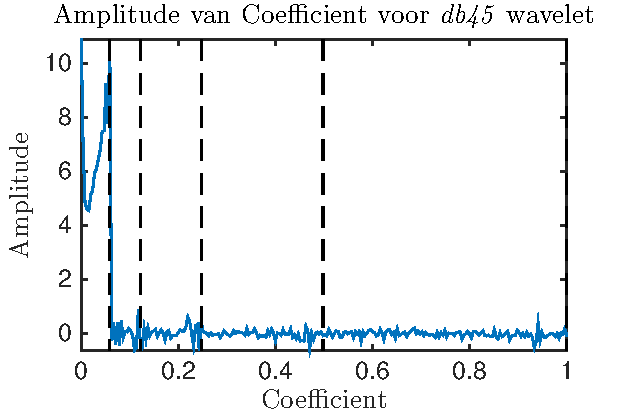
\includegraphics[width=\textwidth]{../src/denoising/db45_Noise/coef_exp_db45_4_noise_10}
        \caption{Met tekst beschadiging}
        \label{fig:tiger}
    \end{subfigure}
    ~ %add desired spacing between images, e. g. ~, \quad, \qquad, \hfill etc. 
    %(or a blank line to force the subfigure onto a new line)
    \begin{subfigure}[b]{0.45\textwidth}
        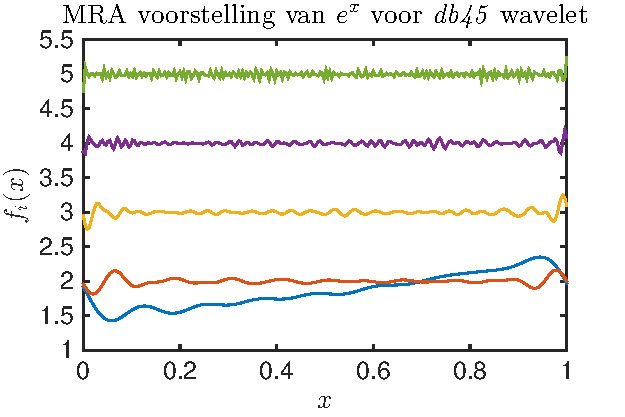
\includegraphics[width=\textwidth]{../src/denoising/db45_Noise/MRA_exp_db45_4_noise_10}
        \caption{Na de reconstructie}
        \label{fig:mouse}
    \end{subfigure}
    \caption{Pictures of lena}\label{fig:exp_Noise_noise_10}
\end{figure}






\begin{figure}
\centering
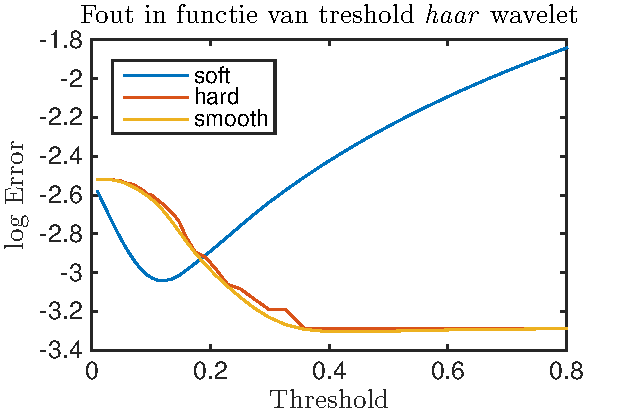
\includegraphics[width=0.7\linewidth]{../src/denoising/error_1d/error_exp_haar_10}
\caption{}
\label{fig:error_exp_haar_10}
\end{figure}
\begin{figure}
\centering
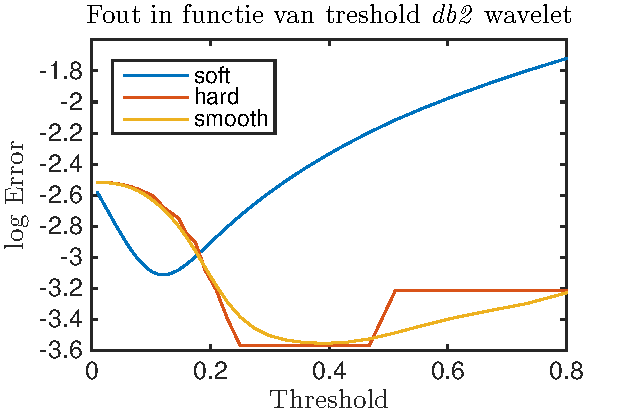
\includegraphics[width=0.7\linewidth]{../src/denoising/error_1d/error_exp_db2_10}
\caption{}
\label{fig:error_exp_db2_10}
\end{figure}
\begin{figure}
\centering
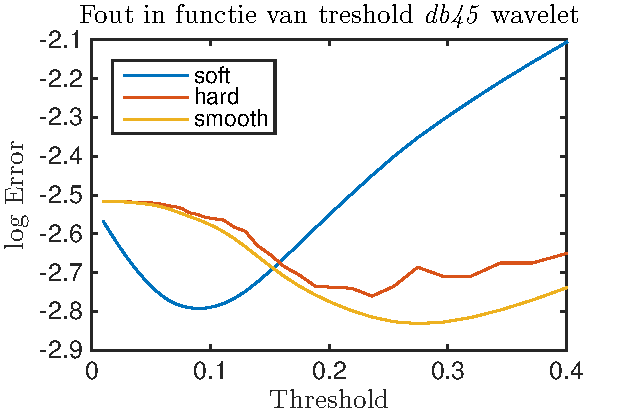
\includegraphics[width=0.7\linewidth]{../src/denoising/error_1d/error_exp_db45_10}
\caption{}
\label{fig:error_exp_db45_10}
\end{figure}


\begin{figure}
\centering
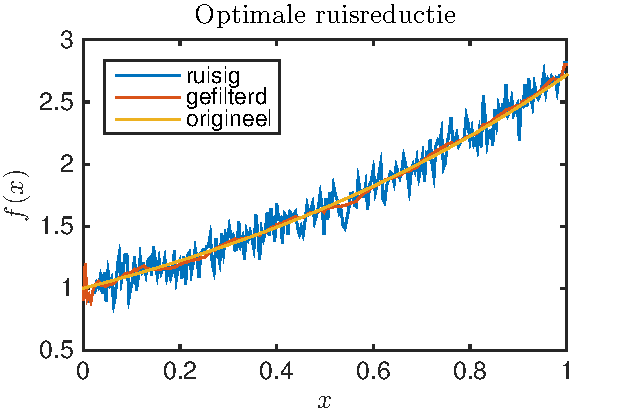
\includegraphics[width=0.7\linewidth]{../src/denoising/error_1d/Optimale_ruisReductie}
\caption{}
\label{fig:Optimale_ruisReductie}
\end{figure}

\begin{figure}
\centering
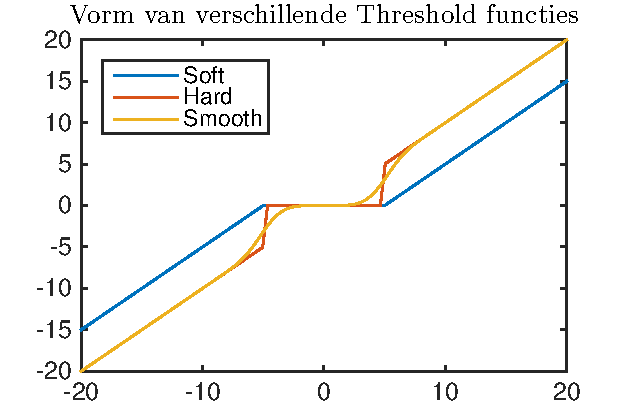
\includegraphics[width=0.7\linewidth]{../src/denoising/error_1d/Threshold}
\caption{}
\label{fig:Threshold}
\end{figure}






\subsection{Moving on to images}

Voor de ruis experimenten op afbeelding is er steeds met een zelfde ruis gewerkt.
De ruis was gaussische verdeeld met een standaard afwijking van 0.1.
Verder werd de ingelezen afbeelding eerst genormaliseerd.
Op deze manier is het eenvoudiger resultaten tussen verschillende afbeeldingen te vergelijken en een normalisatie komt ook meestal ten goede van de conditionering.

\subsubsection{Implementatie van ruis reductie algoritme}


De eenvoudigste manier voor ruis uit een afbeelding te halen aan de hand van een wavelet transformatie is door exact de zelfde strategie toe te passen als in het 1 dimensionaal geval.
Dit houd in dat eerst de wavelet coefficienten worden bepaald voor de ruisige afbeelding.
Nadien worden deze coefficienten met een threshold functie op een niet lineaire manier gefilterd.
De laatste stap is dan de afbeelding reconstrueren aan de hand van de gefilterde coefficienten.
Een concrete implementatie van dit algoritme is terug te vinden in de \textbf{appendix}.

\subsubsection{Verschil in threshold functies}

Voor een goed beeld te krijgen van de invloed van de threshold functie op de ruisreductie hebben we de kwaliteit van de ruisreductie vergeleken voor de verschillende threshold functies.
Voor elke threshold functie werden er een aantal threshold parameters getest.
Een voorbeeld resultaat van zo een test is te zien in Figuur \ref{fig:snr_image_bior6}.
In deze figuur is de SNR waarden geplot voor  verschillende threshold waarden en voor verschillende threshold functies.
Uit deze afbeelding is af te leiden dat zachte threshold functie het beste resultaat opleverd voor de ruisreductie.
In Figuur \ref{fig:snr_image_bior6} werd gebruik gemaakt van de biorthogonale wavelet van orde 6,8.
Voor de meeste andere transformaties werden gelijkaardige resultaten bekomen.
Uit alle tests besluiten  we dat de zachte threshold functie de beste ruisreductie oplevert.


\begin{figure}
\centering
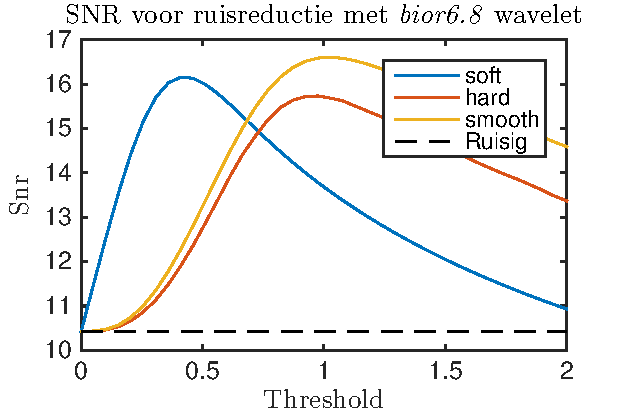
\includegraphics[width=0.7\linewidth]{../src/denoising/image/snr_image_bior68_30.pdf}
\caption{}
\label{fig:snr_image_bior6}
\end{figure}


\subsubsection{Optimale threshold bepalen(met vals spelen)}

Uit het vorige experiment hebben we kunnen besluiten dat in alle gevallen de zachte threshold functie de beste denoising geeft.
Een tweede resultaat dat opviel was dat de SNR curves steeds gladde curves bleken te zijn voor de zachte threshold functie.
Door het gladde karakter van deze curve is het gebruik van een optimalisatie routine voor de SNR costfunctie makkelijk te implementeren.
De cost functie is als volgt gedefini\"eerd in matlab.
\begin{verbatim}
costFun = @(T) -snr_den(An,A,Nb_levels,wname,@(x) SmootThresh(x,T));
\end{verbatim}
Dit is een functie in de parameter \verb|T|, dit is de waarden van de threshold.
\verb|An | is de ruizige afbeelding, \verb|A| de originele afbeelding, \verb|Nb_levels| het aantal niveaus van de transformatie, \verb|wname| de naam van de wavelte transformatie en \verb|@(x) SmootThresh(x,T)| de threshold functie.
Merk op dat voor de berekening van de SNR waarden de originele afbeelding moet gekend zijn (Vals spelen).
Door gebruik te maken van de optimalisatie routine \verb|fmincon| kan de optimale waarden voor de threshold snel worden gevonden.
\begin{verbatim}
[opt_thres,opt_snr] =fminunc(costFun,0.2);
\end{verbatim}
Deze methode convergeerde steeds, soms was de convergentie naar een negatieve waarde van de threshold.
Dit is geen probleem aangezien de threshold functie symmetrisch is in de threshold parameter.

Een voorbeeld resultaat van de optimale ruis onderdrukking is gegeven in figuur \ref{fig:optimaleRuisBIOR}.
In deze figuur is opnieuw de biorthogonale wavelet van orde 6,8 gebruikt.


\begin{figure}
    \centering
    \begin{subfigure}[b]{0.45\textwidth}
        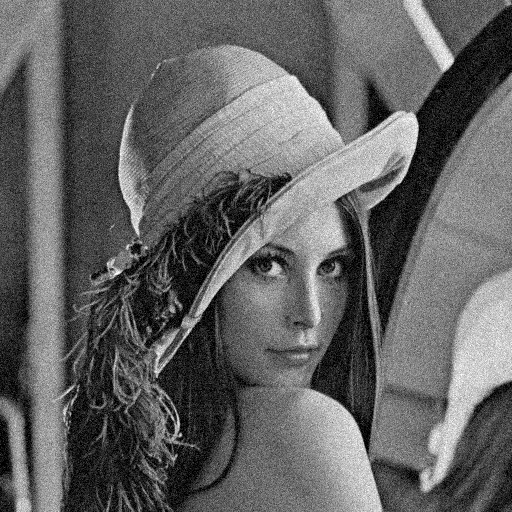
\includegraphics[width=\textwidth]{../src/denoising/image/lenaNoise_bior68.png}
        \caption{Met tekst beschadiging}
        \label{fig:tiger}
    \end{subfigure}
    ~ %add desired spacing between images, e. g. ~, \quad, \qquad, \hfill etc. 
    %(or a blank line to force the subfigure onto a new line)
    \begin{subfigure}[b]{0.45\textwidth}
        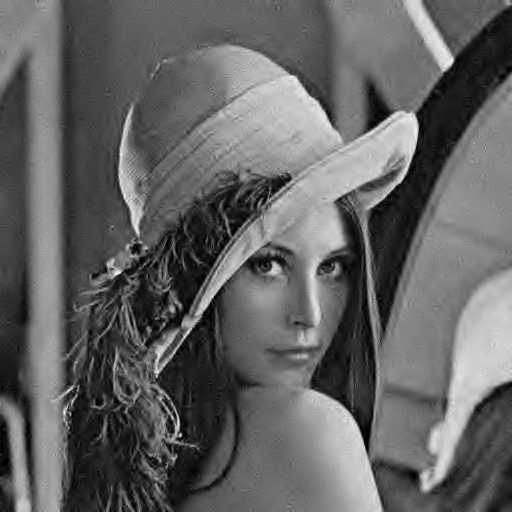
\includegraphics[width=\textwidth]{../src/denoising/image/lenaDen_bior68.png}
        \caption{Na de reconstructie}
        \label{fig:mouse}
    \end{subfigure}
    \caption{Pictures of lena}\label{fig:optimaleRuisBIOR}
\end{figure}


\subsubsection{Optimale threshold bepalen(zonder vals spelen)}



\subsubsection{Beste strategie}




\subsection{Redundante wavelet transformatie}


De redundante wavelet transformatie voor twee dimensionale foto's kan gebruikt worden via het commando \verb|swt2|.
Dit geeft als resultaat een drie dimensionale array terug met dimensies $ H\times L \times N $, waarbij $ H, L $ respectievelijk de hoogt in pixels en de breedte in pixels van de foto is.
De reconstructie van een ruizige foto kan met behulp van volgende twee lijnen code.
\begin{verbatim}
swc = swt2(X,N,wname);
Y = iswt2(thresHold(swc),wname);
\end{verbatim}
Nadien kan de fout tussen de originele afbeelding $ X $ en de gereconstrueerde foto $ Y $ worden bepaald zoals voorheen.
Dit kan nadien opnieuw worden gebruikt in een optimalisatie routine.

\subsubsection{Resultaten}

Het beste resultaat voor de denoising van afbeeldingen werd bekomen met de redundante wavelet transformatie.
Als kost functie werd de afstand tot de originele afbeelding genomen.
Als threshold functie werd er gekozen voor de zachte threshold.
Hierbij werd de threshold waarden bepaald met behulp van \verb|fmincon|.
Op deze manier werd er een SNR van maximaal 13.85 bereikt waarbij de origine beschadigde foto een SNR van 8.30 dB had.
Dit resultaat is weergegeven in Figuur \ref{fig:redundant}


\begin{figure}
    \centering
    \begin{subfigure}[b]{0.45\textwidth}
        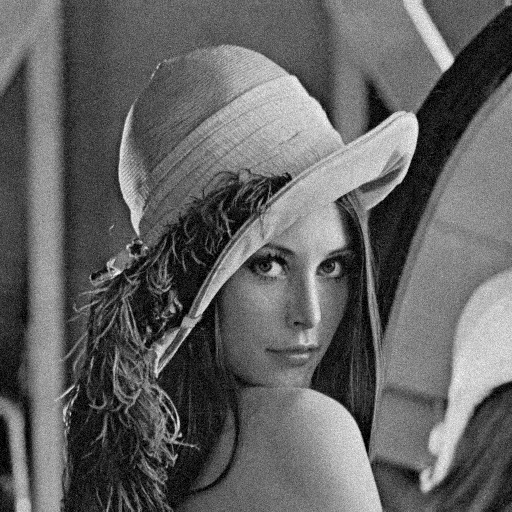
\includegraphics[width=\textwidth]{../src/denoising/redundant/redundant_noise}
        \caption{Beschadigde foto met SNR van 8.30 dB }
        \label{fig:redundant_noise}
    \end{subfigure}
    ~ %add desired spacing between images, e. g. ~, \quad, \qquad, \hfill etc. 
    %(or a blank line to force the subfigure onto a new line)
    \begin{subfigure}[b]{0.45\textwidth}
        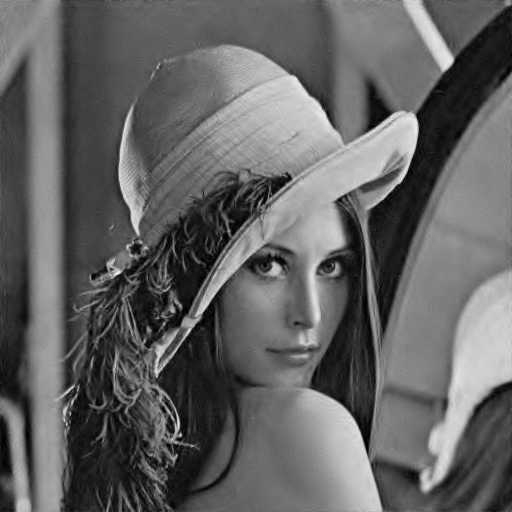
\includegraphics[width=\textwidth]{../src/denoising/redundant/redundant_fixed}
        \caption{Reconstructie met SNR van 13.85 dB}
        \label{fig:redundant_fixed}
    \end{subfigure}
    \caption{Resultaat voor reconstructie van ruizige foto aan de hand van  \textit{db6} wavelet met orde 5. Bij de reconstuctie werd er gebruik gemaakt van de redundante wavelet transformatie. Als threshold functie werd de zachte functie gebruikt. De threshold parameter werd optimaal gekozen aan de hand van een optimalisatie routine. }\label{fig:redundant}
\end{figure}










\subsubsection{Rooster ruis}

















